\documentclass[oneside,a4paper]{article}

% ========== Preamble (packages, definitions etc.) ==========

\usepackage[utf8]{inputenc}
\usepackage{graphicx}
\usepackage{xcolor}
\usepackage{amsmath, amsthm, amssymb}
\usepackage{csquotes}
\usepackage{hyperref}
\usepackage{listings}
\usepackage{lmodern}
\usepackage{float}
\usepackage{braket}

\setlength{\parskip}{\baselineskip}

%\newcounter{questionnum} \setcounter{questionnum}{0}
%\newcommand{\question}[1]{%
%  \refstepcounter{questionnum}%
%  \paragraph{Question~\arabic{questionnum}:}{\emph{#1}}}

\newcommand\filltoend{\leavevmode{\unskip
  \leaders\hrule height.5ex depth\dimexpr-.5ex+0.4pt\hfill\hbox{}%
  \parfillskip=0pt\endgraf}}

\newcommand{\problem}[2]{%
	\vspace{-0.7em}
	\hspace{0.02\textwidth}
	\begin{minipage}[t][][b]{0.95\textwidth}
		{\bf \hspace{-0.015\textwidth}\makebox[7.5em][l]{{#1} ~~\filltoend}}%
		\hspace{1.2mm}{\it #2}%
	\end{minipage}
}

\lstset{ % Set the default style for code listings
	numbers=left, 
	numberstyle=\scriptsize, 
	numbersep=8pt,
	basicstyle=\scriptsize\ttfamily,
	keywordstyle=\color{blue},
	stringstyle=\color{red},
	commentstyle=\color{green!70!black},
	breaklines=true,
	frame=single, 
	language=C++,
	captionpos=b,
	tabsize=4,
	showstringspaces=false
}

\graphicspath{ {res/} }

% ========== Title page ==========

\title {
	
\includegraphics[width=0.6\textwidth]{UU_logo.pdf}\\[1em]
	Cryptology \\
	Report\\[1em]
	%\\[3em]
	Quantum cryptography: Public key distribution and coin tossing
}

\author{
		Hendrik Bierlee \and
		Nodari Kankava
}

\begin{document}



\maketitle
\thispagestyle{empty} % Removes page number for front page
\pagebreak

\newcounter{qcounter}
\setcounter{qcounter}{1}
\newcommand{\question}[1]{\par\vspace{10px}\noindent\textbf{Question \theqcounter \stepcounter{qcounter}:} \emph{#1}\vspace{0.5em}\\\noindent}


% ========== Document contents ==========
\section{Introduction}


\subsection{Problem statement of key-distribution} \label{sec:key-dist-problem}
Key distribution is one of the main issues in cryptography. In a scenario where two parties want to establish a secure communication channel, first they need to agree on a shared secret key. This is an issue for symmetric cryptography protocols, where cryptographic keys has to be securely shared between sender and receiver. Easy key distribution becomes even more important when frequent key change is required or number of participants in communication increases.

\subsection{Classical solution to the public key distribution}
Public key cryptography allows secure distribution of secret keys between parties who don't share initial secret information. The Diffie–Hellman key exchange protocol~\cite{diffie1976new} allows two parties to agree on a shared secret key. This protocol is frequently used in systems that also achieve forward secrecy because of its fast key generation. The Diffie-Helman key exchange is considered secure, until the efficient algorithm to compute discrete logarithm is found.


Classic information theory assumes that communication can be eavesdropped either passively or actively. There is no protection against copying transmitted information. Communicating parties can verify with high degree of confidence that exchanged message was not modified, but they should operate under the assumption that information was most probably copied.
Another major advantage of public key cryptography is message verification and non-repudiation.

\subsection{Problem statement of the remote coin-flip problem}
The `coin-flip by telephone' problem was first described in 1981~\cite{blum1981coin}: two distrusting parties, Alice and Bob, want to play a remote game without a third party where both have an equal win-chance, and where neither can cheat.

\subsubsection{Classical solution to the remote coin-flip problem}
In the same paper, the problem was solved by constructing a one-way function $f$ which is two-to-one, meaning that one can have a pair of inputs $x$ and $y$ that map to the same value $f(x)=f(y)$.
An example of such a function is $f(x) =|1/x|$, because every allowed input $x$ has a counterpart $-x$ that $f$ maps to the same value (except for $0$, which is undefined).
Furthermore, $x$ and $y$ have some distinguishing property, for instance, $x$ is always even and $y$ is always odd. Because of the one-way nature of $f$, Alice can randomly select $x$ but it is computationally impossible for her to also find out the corresponding $y$.

After selecting $x$, Alice sends $f(x)=c_{\text{Alice}}$ to Bob (her \textit{commitment} to $x$), and from $f(x)$ Bob cannot know whether Alice used $x$ or $y$.
\footnote{
    This idea is reminiscent of a zero-knowledge proof~\cite{goldwasser1989knowledge}, where one party proves they posses certain information without revealing to the other side what that information is.
    Alice proofs to Bob she committed to one of two choices without revealing her actual choice.
}
So, Bob can proclaim a guess to Alice with a 50\% chance of getting it right.
Subsequently, Alice can claim victory or defeat and proof her original choice of $x$ by sending $x$ to Bob.
Bob can verify the claim by recognising that $x$ is in fact even, and by computing $f(x)=c_{\text{Alice}}$.
Alice does not possess $y$, so she cannot possibly cheat by sending Bob an odd value that $f$ maps to $c_{\text{Alice}}$.

A benefit to this problem is that if the messages between Alice and Bob are signed, any attempt at cheating on the part of Alice (say she sends $x'$ such that $f(x') \neq c_{\text{Alice}}$) can be proved to a judge.

\subsection{Need for new solutions}
Many cryptography methods are founded on the assumption that some procedures, such as prime factorisation, are computationally hard, i.e. $P \neq NP$.
A prime example of this is prime factorisation, or computing discrete logarithms.
However, this assumption may yet be invalidated by breakthroughs in algorithm design, or, more on topic, the introduction of quantum computing that can execute algorithms such as Shor's algorithm, which can do prime factorisation in polynomial time~\cite{bernstein2017post}.
In the next section, we will summarise the quantum methods for solving the problems, which rely on fundamental properties of physics for security.

\section{Problem solution}
Before presenting the solutions for public-key exchange and remote coin-flipping, we briefly introduce some of the fundamental properties of photons that will be used in both solutions.

In our following discussion, we assume \emph{good} but not \emph{perfect} quantum hardware (when it comes to the ability to pick out, send, receive and measure individual photons).
Perfect hardware would enable cheating the coin-flip with the EPR effect, as discussed in section~\ref{sec:cheating-epr}.

\subsection{The behaviour of polarised photons}
Light exists of individual photon particles, which can be polarised at any angle using polarising filters.
Four of these polarisation axis are important to us: two rectilinear (0 degrees, 90 degrees) and two diagonal (45 degrees, 135 degrees).
To measure the orientation of a polarised photon, one can again use polarising filters.
If the orientation (or basis) of the filter matches the orientation of the photon, the photon will pass through, and if the filter is orthogonal to the photon, the photon will not pass through.
In other words, rectilinear photons can be measured accurately 100\% of the time (deterministically) if one uses the `correct', rectilinear filter, since the difference in angle between photon and a filter at 0 degrees is always either 0 or 90 degrees.

But suppose the difference is 45 degrees, such as is always the case when you try to measure rectilinear photons with a `wrong', diagonal filter. 
It happens that the probability of photons passing through this filter is exactly 50\%, so the measurement will tell you exactly nothing about the original polarisation.
Photons that did pass through now have the same polarisation as the filter, so re-measuring them tells you nothing about their original orientation.
Furthermore, we cannot simply clone photons and perform multiple measurements.
Essentially, you only get one chance to measure a photon, and even though there is theoretically infinite information in a photon (if the polarisation is on a continuous spectrum), measurement will only yield one bit of information.

\subsection{Quantum key distribution}
In the quantum key distribution protocols, a quantum channel is used to exchange random bits between two parties who haven't initially shared any secret information and then continue conversation using a classic communication channel. As soon as both parties share random bits using a quantum channel, they will be able to verify that quantum key exchange was not disturbed and be able to agree to use the shared secret bits to encrypt classic communication channel.

Unlike digital communications that can be monitored and copied, transmissions inside a quantum communication channel cannot be copied or observed without randomly and uncontrollably changing the state, therefore any disturbance will be evident. If communicating parties detect that their exchange was disturbed they will try again to securely share enough random bits using a quantum channel to have a guarantee with high probability that their communication is secure.


The protocol for a quantum key exchange is as follows:

Using a quantum channel:
\begin{enumerate}
    \item Alice chooses random bit-string, encodes each bits as polarised photons, switching randomly between rectilinear and diagonal bases and sends polarised photons to Bob.
    \item Bob independent of Alice, randomly chooses what bases to use to measure photons (rectilinear or diagonal polarisation).
\end{enumerate}

Using a classic channel (with the assumption that it could be monitored, but those messages can't be changed or altered):

\begin{enumerate}
    \setcounter{enumi}{2}
    \item Bob reveals for each photon what basis he used to measure (rectilinear or diagonal).
    \item Alice reveals which basis were correct.
    \item Alice and Bob use the correct bits to generate a key for use in classic communication channel.
\end{enumerate}

Because photons have to be measured using random choice of rectilinear or diagonal basis, any measurement by an eavesdropper will alter the message Bob gets and subsequently produce disagreement between Alice and Bob on bits that they should agree on.

\subsection{The quantum remote coin-flip protocol}
The protocol for a quantum remote coin-flip is as follows:
\begin{enumerate}
	\item
		Alice chooses at random a secret basis (rectilinear or diagonal) and encodes a secret, random bit-string of decent length as polarised photons using her chosen basis.
		She sends over the photons to Bob on a quantum channel.
	\item
		To win, Bob has to guess Alice's choice of basis.
		But when Bob receives the photons, he does not know how to measure them deterministically to find out their polarisation.
		The best he can do is switch bases randomly and independently for each photon, so that he at least ends up with a half-filled rectilinear measurement table and a half-filled diagonal measurement table, one of which is 100\% correct and the other is 50\% correct.
		With nothing to go on, Bob has to make a random guess to Alice as to the original basis.
	\item Alice reveals her basis, and sends over the original bit-string on a classical channel.
	\item Bob can verify Alice's choice, because he can confirm that the elements of the bit-string matches up 100\% with the corresponding measurement table.
\end{enumerate}

Like in the classical solution, the key is that one party has to send a commitment to their choice to the other party, without revealing the choice itself.

\section{Benefits and drawbacks of the solutions}
Here we discuss the benefits and drawbacks to the solution.

\subsection{Advantages of the quantum remote coin-flip protocol}

\subsubsection{Impossibility of cheating}
The protocol is protected against cheating by the laws of physics, instead of by computational hardness:

\begin{itemize}
	\item Given the polarised photons, Bob cannot guess the basis of the polarisation with a probability greater than $1/2$.
	\item Alice has to provide the measurement results of the table with the basis she supposedly picked: if she lies about the basis (because Bob guessed it correctly), she would have to guess the contents of the other table.
	If $n$ photons were sent, the probability that she can perfectly match the table is $\frac{1}{(n/2)^2}=\frac{4}{n^2}$.
	Getting even one measurement wrong would expose Alice as a cheater.
	\item Alice could send a mix of rectilinear and diagonal photons, but then she would not be able to verify either table.
\end{itemize}

\subsection{Common disadvantages and possible attacks for quantum key distribution and coin-tossing}
As mentioned in section~\ref{sec:key-dist-problem}, classic information theory assumes that digital communications can be passively monitored. Quantum information theory guarantees that communication cannot be passively monitored and forces the adversary to be active and detectable. However there are possible drawbacks.

\subsubsection{No non-repudiation}
One of the issues with quantum communication is that there is no way of verifying who sent the individual photons. Digital signatures cannot be created with quantum cryptography. There is no such thing as signing photons. Related to this issue is that an eavesdropper can try to suppress communications by introducing noise into a channel or just by trying to measure photons. This is a threat to availability and integrity, but not to the confidentiality.
Also in case of quantum coin-flip Alice or Bob could deny that the coin-flip happened (and the other would not be able to prove to a judge that it did happen).

\subsubsection{Generating random bit-strings}
The bit-string that Alice encodes needs to be generated by a cryptographically secure pseudo-random number generator.
In a post-quantum world, a CSPRNG that relies on prime-factorisation (such as a RSA generator) would be compromised, so it obviously should not be used in an implementation of this protocol.
%TODO ref to slides / RSA generator?
Maybe Alice should just measure rectilinear photons diagonally, instead.

\subsection{Disadvantages of the quantum key distribution}
\subsubsection{Theoretical attacks}
More sophisticated attacks involve quantum phenomena that have not yet been demonstrated as possible but exist as a theoretical thought experiment. In this case if an adversary can clone or multiply photons he can measure them in multiple bases and choose correct ones after Alice and Bob share correct bases in public channel.

\subsection{Disadvantages of the quantum remote coin-flip protocol}

\subsubsection{Need for quantum hardware} %TODO probably for general to both
Even though a version of the quantum remote coin-flip has been performed experimentally by researchers at the Laboratory for Communication and Processing of Information (LTCI) in Paris~\cite{pappa2014experimental}, there is no prediction for when quantum hardware will become available.
This is also good news, because it means that for now we can still rely on computational hardness to safeguard the classical solution.
More generally, one could state that quantum solutions will become useful on the same day that classical solutions will be compromised.

\subsubsection{Possibility of cheating}
\label{sec:cheating-epr}
In theory, Alice can cheat by using the Einstein-Podolsky-Rosen effect, which implies that pairs of polarised photons can be created which always collapse to opposite directions (regardless of in which basis they are measured).
Alice could encode the bit-string in such pairs, send one photon of each pair to Bob and keep the other.
If Bob then guesses, say, rectilinear, she can measure her photons in the diagonal basis, thus being able to match the results of Bob's diagonal table, pretending to have used diagonal encoding all along and verifying her `win'.

However, storing and measuring the twin photons with 100\% accuracy is likely impossible in practice, even with good quantum hardware.

\section{Implementation of a quantum remote coin-flip protocol simulation}
For those who can't wait until quantum computers become commercially available, the Microsoft Q\#~\cite{qsharp} project provides a quantum development kit for expressing quantum algorithms and running simulations of them on a classical machine.
With this, we implemented (a simulation of) the quantum remote coin-flip protocol~\cite{quantum-coin-toss-repo}.
The end-product is a simulation in two ways: obviously, no actual qubits were used, and secondly, since Q\# does not provide a way to simulate a quantum channel, the communication between Alice and Bob takes place in one process.

To implement the protocol, we need to translate photons, polarisation filter, etc. over to the world of quantum computing.

\subsection{Qubits and operating on them}
Photons are one way to achieve quantum behaviour, but in quantum computing, the implementation (be it photons or otherwise) is abstracted away behind the concept of qubits, which uses linear algebra as foundation.
A qubit is represented as a unit vector $\vec{q}=\begin{pmatrix} \alpha \\ \beta\end{pmatrix}$ where $\alpha, \beta \in \mathbb{C}$ and $||\vec{q}||=1$.
Here we have four examples of qubits, along with their more convenient Dirac notations:

\begin{equation}
    \label{eq:qubits}
    \begin{pmatrix} 1 \\ 0\end{pmatrix} = \ket{0}, \quad
    \begin{pmatrix} 0 \\ 1\end{pmatrix} = \ket{1}, \quad
    \begin{pmatrix} \frac{1}{\sqrt{2}} \\ \frac{1}{\sqrt{2}}\end{pmatrix} = \ket{+}, \quad
    \begin{pmatrix} \frac{1}{\sqrt{2}} \\ \frac{-1}{\sqrt{2}}\end{pmatrix} = \ket{-}.
\end{equation}

Qubits can be manipulated using linear transformations, such as the negation operation $X$ and the Hadamard gate operation $H$:

\begin{equation}
    X = \begin{pmatrix} 0 & 1 \\ 1 & 0 \\\end{pmatrix}, \quad
    H = \begin{pmatrix} \frac{1}{\sqrt{2}} & \frac{1}{\sqrt{2}} \\ \frac{1}{\sqrt{2}} & \frac{-1}{\sqrt{2}} \\\end{pmatrix}.
\end{equation}

With simple linear algebra we can easily transform our qubits in equation~\ref{eq:qubits} from one into another using $X$ and $H$:

\begin{equation}
    \label{eq:operations}
    X(\ket{0}) = \ket{1},
    \quad H(\ket{0})=\ket{+},
    \quad H(\ket{1})=\ket{-}.
\end{equation}

Since qubits are (unit) vectors, they can be seen as points on the surface of a unit sphere, the so-called Bloch sphere~\cite{bloch1946nuclear}.
For our purposes, we don't need qubits with imaginary numbers, so we stay within one slice of the sphere: a unit circle.
In figure~\ref{fig:unit-circle}, we can see the effects of using $X$ and $H$ on qubits in different states.

\begin{figure}
    \centering
    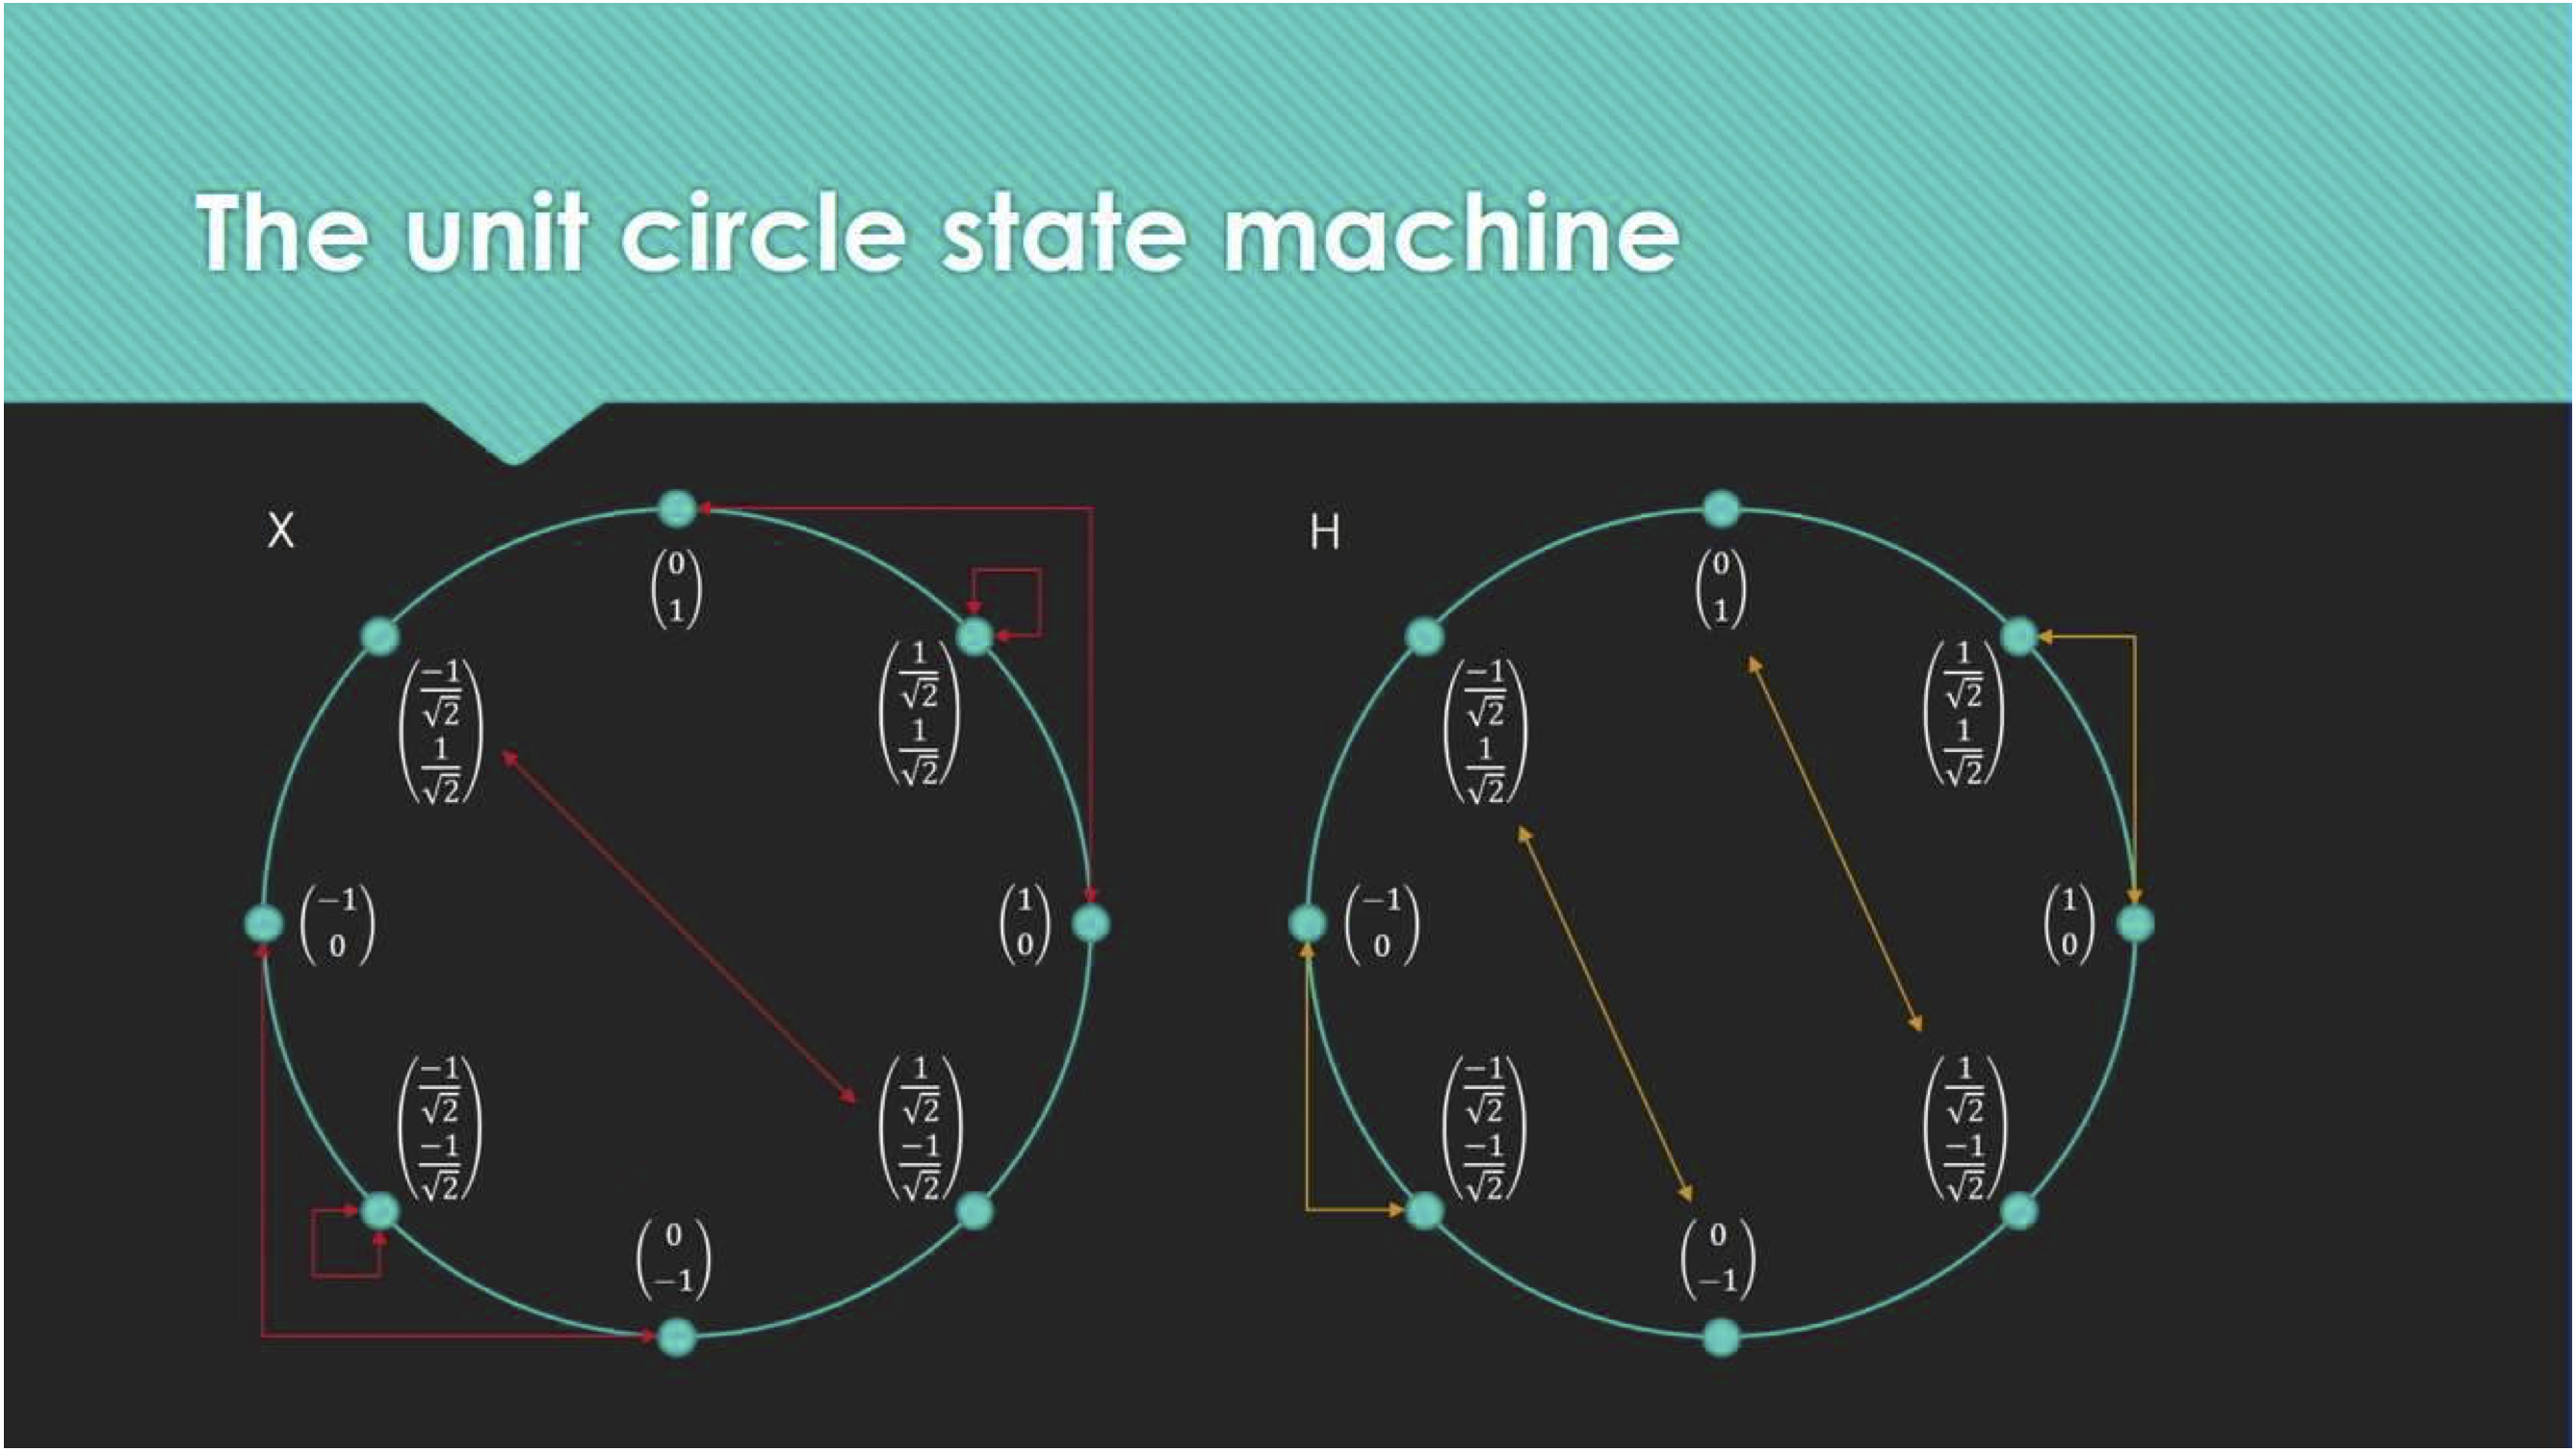
\includegraphics[width=\linewidth]{microsoft-quantum-coding-unit-circle}
    \caption{The unit circle state machine, displaying the effects of $X$ and $H$ operations. Taken from the supporting slides of a Microsoft talk: \emph{`Quantum Computing for Computer Scientists'}~\cite{quantum-computing-talk}.}
    \label{fig:unit-circle}
\end{figure}


\subsection{Measuring qubits}
The $\alpha$ and $\beta$ values determine the superposition or quantum state of the qubit, but we cannot obtain these values directly.
Instead, we have to measure $\vec{q}$, and the only possible outcomes are either $0$ or $1$, ie. a classical bit (or cbit).
The result of a measurement $M$ is probabilistic, and depends on the value of $\alpha$ and $\beta$:

\begin{equation}
    \label{eq:measuring-distribution}
    P(M=0) = |\alpha|^2,
    \quad P(M=1) = |\beta|^2.
\end{equation}

Just like with photons, the basis in which we measure can be varied, so we have to specify that too: in this case using the Pauli measurements. 
Two Pauli measurements are of importance: Pauli Z and Pauli X.
Measuring Pauli Z,~$\ket{0}$ always results in~$0$ and ~$\ket{1}$ always in~$1$.
However, when measuring Pauli Z of either~$\ket{-}$ or~$\ket{+}$ we get an uniformly random outcome of $0$ and $1$. This is in line with the above equation~\ref{eq:measuring-distribution}.

With Pauli X, things are turned around: measuring Pauli X of~$\ket{-}$ and~$\ket{+}$ deterministically leads to~$0$ and~$1$ (respectively), but when measuring Pauli X of~$\ket{0}$ and~$\ket{1}$ there is a 50\% chance of~$0$, 50\% chance of~$1$.
On a side-note, measuring Pauli X of~$\vec{q}$ is equivalent to first performing~$H$, and then measuring Pauli Z.

Just like in other quantum systems, no re-measurements is possible (the qubit is said to have collapsed to one of two states) and no cloning is possible (which prevents statistical analysis of a single qubit).

\subsection{From photons to qubits}
With this foundation of quantum computing, we are ready to define the quantum computing equivalent of the quantum remote coin-flip protocol:

\begin{itemize}
    \item A photon with a polarisation axis of~$\theta$ degrees can be represented as a qubit with $\alpha=\cos{\theta}$ and $\beta=\sin{\theta}$.
    Specifically, $\ket{0}$ and $\ket{1}$ are our rectilinearly polarised photons, and ~$\ket{-}$ and~$\ket{+}$ are the diagonal ones.
    \item To encode a bit from a bit-string, we can start from the $\ket{0}$ qubit and use the $X$ and $H$ operations (see equations~\ref{eq:operations}) to achieve any of the four polarisations.
    \item To measure with a rectilinear or diagonal filter, we can measure Pauli Z or Pauli X, respectively.
\end{itemize}


\subsection{Q\# code sample}
The following Q\# operation performs the encoding, from a $\ket{0}$ qubit, rectilinear/diagonal basis and 0/1 bit:

\begin{lstlisting}[caption={\texttt{Operations.qs}}]
operation Encode (qubit : Qubit, rectilinear : Bool, bit : Bool) : Unit {
    if (rectilinear && not(bit)){
        // do nothing, qubit is already |0>
        return (); // since there is no `else if` statement in Q#, we return after each if-statement
    }
    if (rectilinear && bit) {
        X(qubit);   // |1>
        return ();
    }
    if (not(rectilinear) && not(bit)) {
        H(qubit);   // |+>
        return ();
    }
    if (not(rectilinear) && bit) {
        X(qubit);   // |1>
        H(qubit);   // |->
        return ();
    }
}
\end{lstlisting}

\bibliography{sources}
\bibliographystyle{acm}

\end{document}
